%% PAQUETES
\usepackage[utf8]{inputenx}
\usepackage[spanish]{babel}
\usepackage{amsmath}
\usepackage{amsthm}
\usepackage{amssymb}
\usepackage{amsfonts}   
\usepackage{pifont}     % Para tickYes y tickNo
\usepackage{graphicx}
\usepackage{epsfig}
\usepackage{pdflscape}
\usepackage{enumerate}
\usepackage{color}
\usepackage{beamerfoils}
\usepackage{beamerprosper}
\usepackage{xspace}
\usepackage{booktabs}
\usepackage{multicol}
\usepackage{multirow}
\usepackage{tikz}
\usepackage{pgflibraryshapes}
\usepackage{wasysym}
\usepackage{float}
\usepackage{listings}

%% CONFIGURACIÓN DE TIKZ
% Librerías cargadas
\usetikzlibrary{arrows}
%\usetikzlibrary{calc,fadings,decorations.pathreplacing,arrows,intersections,
%    decorations.markings,external,shapes}

% Configuración de Tikz y Pgfplot
\tikzset{%
    >=stealth, % option for nice arrows
    inner sep=0pt,%
    outer sep=3pt,%
    mark coordinate/.style={inner sep=0pt,outer
    sep=0pt,minimum size=3pt,
    fill=black,circle}%
    }

% Librerías de tiKz
    %\usetikzlibrary{}

    % Define block styles
\tikzstyle{io} = [trapezium,trapezium left angle=70,trapezium right angle=-70,
  minimum height=0.9cm, draw, fill=blue!20, text width=4.5em, 
  text badly centered, node distance=2cm, inner sep=0pt]
\tikzstyle{decision} = [diamond, draw, fill=blue!20, text width=5.5em, 
  text badly centered, node distance=2cm, inner sep=0pt]
\tikzstyle{block} = [rectangle, draw, fill=blue!20, text width=5em, 
  text centered, rounded corners, minimum height=4em]
\tikzstyle{line} = [draw, -latex']
\tikzstyle{cloud} = [draw, ellipse,fill=red!20, node distance=2cm, 
    minimum height=2em]


%% TEMAS BASE
\usefonttheme{structurebold}
\usecolortheme{orchid}
\usetheme[hideothersubsections,left,width=.13\textwidth]{Goettingen}

% \usetheme{Boadilla}
% \setbeamertemplate{headline}{
%   \begin{beamercolorbox}{section in head/foot}
%   \vskip2pt\insertnavigation{\paperwidth}\vskip2pt
%   \end{beamercolorbox}
%   \includegraphics[width=\paperwidth]{images/ucm_logo}
% }
% \usecolortheme{lily}

\useinnertheme{circles}

\definecolor{ZurichBlue}{rgb}{.255,.41,.884}
\setbeamercolor{alerted text}{fg=ZurichBlue}
\definecolor{Comentario}{rgb}{0.0,0.5,0.0}

%% CONFIGURACIÓN GEENERAL DE HIPERVÍNCULOS
\hypersetup{%
    baseurl={roberto.antolin@forestry.gsi.gov.uk},
    pdftitle={LiDAR},%
    pdfauthor={Roberto Antol\'{i}n S\'anchez},%
    pdfcreator={Roberto Antol\'{i}n S\'anchez},%
    pdfproducer=PDFLaTeX,%
    pdfsubject={LiDAR data filtering},%
    pdfkeywords={filtros, LiDAR data, formats, repositories, workflow}%
  }

\mode<presentation>{\hypersetup{pdfpagemode=FullScreen}}

%% COMANDOS
% Tipos de datos
\newcommand{\file}[1]{\path{#1}\xspace} %Referencias a ficheros
\newcommand{\extr}[1]{\emph{#1}\xspace} %Palabras extranjeras
\mode<article>{\newcommand{\soft}[1]{\textsf{#1}\xspace} }%Referencias a software
\mode<presentation>{\newcommand{\soft}[1]{\textrm{#1}\xspace} }%Referencias a software
\newcommand{\sigl}[1]{\textsc{#1}\xspace} %Siglas
\newcommand{\nota}[1]{\textcolor{nota}{�#1?}\xspace}
\newcommand{\frametitlee}[1]{\mode<presentation| handout| article:0>{\frametitle{#1}}}
\newcommand{\figuree}[2]{
  \mode<article>{
    \begin{figure}[H]
    \centering
    }
    #1
    \mode<article>{
    \caption{#2}
    \end{figure}
  }
}

% Atajos
\newcommand{\inet}{\extr{Internet}}
\newcommand{\html}{\sigl{html}}
\newcommand{\web}{\extr{web}}
\newcommand{\software}{\extr{software}}
\newcommand{\hardware}{\extr{hardware}}
\newcommand{\tickNo}{\color{red}\ding{55}}
\newcommand{\tickYes}{\color{green!50!black}\checkmark}

%% PREFERENCIAS PARA LISTINGS (código)
\lstdefinestyle{mio}{
  basicstyle=\ttfamily\scriptsize,%
  keywordstyle=\bfseries\color{ZurichBlue},%
  commentstyle=shape\color{green},%
  stringstyle=\color{red!50!black},
}

\lstdefinestyle{latex}
{
language={[latex]tex},
keywordstyle=\color{resalta!50!black},
commentstyle=\color{fondoO!50!green}\itshape
}

\lstdefinestyle{shell}{
  language=sh,
  basicstyle=\ttfamily\scriptsize,%
  morekeywords={lasinfo,lasdiff,lasmerge,las2txt,txt2las,las2ogr,laszip,
    lasview, lasboundary, lasgrid, lasduplicate, lasoverlap,
    las2dem, las2las, lastile, lasground, lasheight, lasclassify},
  keywordstyle=\bfseries\color{ZurichBlue},
  commentstyle=\color{green!35!black}%
}

\lstdefinestyle{grass}{                                                                     
  language=sh,
  basicstyle=\ttfamily\scriptsize,%
  morekeywords={v.lidar.edgedetection,v.lidar.growing,
  v.lidar.correction,v.surf.bspline,v.outlier},
  keywordstyle=\bfseries\color{ZurichBlue},classoffset=1,
  commentstyle=shape\color{green!75!black},%
  morekeywords={GRASS6 (stuttgart):, >}
  keywordstyle=\color{green!50!black}, classoffset=0
}

%
\lstdefinestyle{matlab}{
  basicstyle=\scriptsize\ttfamily,
  breaklines=true,
  commentstyle=\color{Comentario},
  keywordstyle=\bfseries\color{blue},
  language=Matlab,
  %xleftmargin=\parindent,
  identifierstyle=\bfseries
}

\lstset{style=mio,
   tabsize=4,%
   inputencoding=utf8,%latin1,%
   extendedchars=true,%
   breaklines=true,%
   showstringspaces=false,
   backgroundcolor=\color{gray!20!white}
   }

%% DATOS DEL DOCUMENTO
\title[LiDAR]
    {LiDAR}

\author[R. Antolín]
    {Roberto Antolín Sánchez}

\institute[FR]{
  Investigador y desarrollador \\
  Forest Research \\
  Northern Research Station \\
  Roslin EH25 9SY \\
  \texttt{roberto.antolin@forestry.gsi.gov.uk}\\
}

%% FECHA DE LA PRESENTACIÓN
\date[15-03-2014]{15 de Marzo de 2014}

\AtBeginSection[]
{
  \begin{frame}[shrink=20]
    \frametitle{Table of Contents}
    \tableofcontents[currentsection,hidesubsections]
  \end{frame}
}

\begin{document}
%\includeonlyframes{cc}
%intro3,intro4,funciona,ventajas1,ventajas2,ventajas3
%desventajas,miktex,miktex2,editores,otrasherr
%%================================================================== Logo On/Off
\LogoOff

%==================================================================FRONT PAGE AND TOC
% For article only
\mode<presentation:0>{\thispagestyle{empty}\maketitle}

% For presentation only
\mode<presentation| article:0| handout:0>{
    \begin{frame}<article:0>[label=portada]
    \titlepage
    \end{frame}%Fin del frame
}

% For handout only
\mode<handout>{
  \begin{frame}[label=portada]
    \maketitle
  \end{frame}
}

%% TABLE OF CONTENTS
\begin{frame}[label=toc]
    \mode<article:0>{\frametitle{Contents}}
    \mode<presentation>{\small}
    \tableofcontents%[hidesubsections]
\end{frame}

%%==================================================================S INTRODUCTION
\section[ALS]{\textquestiondown Qué es el LiDAR aéreo?}
%%==================================================================Sb
\subsection{Principios}
%%==================================================================F 
\begin{frame}
 \frametitle{Principios del LiDAR aéreo}
 \begin{enumerate}
   \item El LiDAR aéreo (Airborne Laser Scanner, \alert{ALS}) es la combinación de:
    	\begin{itemize}
    	 \item \alert{Escaner Laser}
    	 \item \alert{GPS}, que nos da la posición del sensor.
    	 \item \alert{IMU}, que nos da nuestra orientación del avión.
    	\end{itemize}
   \item La posición con respecto al sensor de un punto en tierra se determina por:
     \begin{itemize}
       \item El \alert{tiempo} que tarda cada impulso desde que es emitido hasta que es recibido.
       \item El \alert{ángulo} medido desde el nadir en el cual ha sido emitido el rayo.
     \end{itemize}
   \item La posición relativa combinada con la posición global (\alert{GPS}) y la orientación (\alert{IMU}) nos permiten calcular las coordenadas (X,Y,Z) en el punto medido en tierra en un sistema de posicionamiento global (WGS84)
 \end{enumerate}
\end{frame}
%%==================================================================Sb
\subsection{Características}
%%==================================================================F
\begin{frame}[label=lidar_charact]
   \frametitle{Características del ALS}
   \begin{enumerate}
     	\item \alert{Alta precisión} tanto en la componente planimétrica como en la altrimétrica
     	\item \alert{Alta resolución} debido a la frecuencia de medición.
     	\item \alert{Monoscópica} y casi \alert{nadiral} $\Rightarrow$ permite observar el terreno incluso en zonas de gran vegetación
   \end{enumerate}
\end{frame}
%%==================================================================Sb
\subsection{Primer y último impulso}
%%==================================================================F 
\begin{frame}
  \frametitle{LiDAR}
    \begin{center}
      \only<1>{\includegraphics[width=0.95\textheight]{images/rebote}}
      \only<2>{\includegraphics[width=0.95\textheight]{images/rebotes}}
    \end{center}
\end{frame}
%%==================================================================F
\begin{frame}[label=firstlast1]
    \frametitle{Primer y último impulso}
    \begin{enumerate}
      \item Debido a la divergencia del láser, pueden recibirse \alert{más de un eco} para el mismo rayo.
    	\item Los sensores actuales son capaces de medir al menos dos retornos: \alert{primero} y \alert{último}
    	\item Normalmente se producen por: \alert{bordes} de edificios o \alert{vegetación}
    \end{enumerate}
    \begin{center}
      \includegraphics[height=0.35\textheight]{images/roof}~
      \includegraphics[height=0.35\textheight]{images/tree}
    \end{center}
\end{frame}
%%==================================================================F 
\begin{frame}
    \frametitle{\textquestiondown Para qué sirve?}
    \begin{enumerate}
     \item Una diferencia considerable entre el primer y último impulso puede ser una pista para detectar vegetación y otros objetos: edificios, puentes, tendidos eléctricos...
     \item Los últimos impulsos tienen más probabilidad de ser terreno
     	\begin{itemize}
     	   \item Primer impulso: creación de Modelo Digital de Superficie (\alert{DSM})
     	   \item \'Ultimo impulso: determinación de Modelo Digital del Terreno (\alert{DTM})
     	\end{itemize}
     \item Hay pocas posibilidades de, sin hacer ningún análisis, distinguir entre un punto \alert{objeto} y uno \alert{terreno}.
    \end{enumerate}
\end{frame}
%%==================================================================S
\section[Datos]{Datos LiDAR}
%%==================================================================F
\begin{frame}
  \frametitle{Estándares}
    \begin{center}
      \includegraphics[width=0.75\textwidth]{images/standards}
    \end{center}
  \tiny
  \begin{itemize}
    \item \alert{SITUACIÓN}: Hay 14 estándares diferentes
    \item 14?! Ridículo! Necesitamos desarrollar un estándar universal que cubra todos los posibles casos de uso
    \item \alert{SITUACIÓN}: Hay 15 estándares diferentes
  \end{itemize}
\end{frame}
%%==================================================================F 
\pgfdeclareimage[width=0.7\textwidth]{las}{images/las_format}
\begin{frame}
\frametitle{Estándar binario \emph{LAS} del ASPRS:}
\begin{itemize}
 \item Encabezado público
 \item Registros de longitud variable
 \item Puntos: X, Y, Z, Intensidad, clasificación, dirección de la pasada del vuelo,...
    \begin{center}
  \begin{tikzpicture}
        \pgftext[bottom,left,at={\pgfpointxy{0}{0}}]{\pgfuseimage{las}}
  \end{tikzpicture}
   \end{center}
 \item Para un conversor \alert{abierto} del estándar \emph{LAS}:
\beamergotobutton{\url{http://liblas.org/}}
\end{itemize}
\end{frame}
%%==================================================================F 
\defverbatim[colored]\laszip{
  \begin{lstlisting}[style=shell]
    $ laszip lidar.las lidar.laz
    $ laszip lidar.laz lidar_copy.las
  \end{lstlisting}
}
\begin{frame}
\frametitle{Estándar binario \emph{LAZ}}
\begin{enumerate}
  \item Compresión de archivos .LAS sin \alert{pérdida}
  \item 7\% - 20\% del tamaño del archivo original
  \item Formato LAS comprimido \beamergotobutton{\url{http://www.laszip.org/}}
  \item Ejemplo:
    \laszip
\end{enumerate}
\end{frame}
%%==================================================================F 
\frame[containsverbatim]{%
  \frametitle {Estándar binario SPD}
  \begin{itemize}
    \item Encabezado público
    \item Ficheros indexados
    \item Puntos: X, Y, Z, Intensidad, clasificación, dirección de la pasada del vuelo,...
    \item Procesa datos \alert{\emph{full waveform}}
    \item Página: \beamergotobutton{\url{http://www.spdlib.org/}}
  \end{itemize}
}
%%==================================================================F 
\frame[containsverbatim]{%
  \frametitle {Posible formato ASCII}
  \begin{center}
  \begin{verbatim}
              X         Y        Z
          513628.82 5403190.04 291.40
          513628.85 5403191.47 291.24
          513628.95 5403192.93 294.31
          513628.99 5403194.45 294.17
          513628.97 5403196.05 291.26
          513629.01 5403197.58 291.24
          513629.05 5403199.10 291.25
          513629.09 5403200.53 291.26
                        ...
  \end{verbatim}
  \end{center}
}
%%==================================================================F 
\begin{frame}
  \frametitle{¡Datos LIBRES!}
  \begin{itemize}
    \item \beamergotobutton{\url{http://www.lidar-online.com/products-list.php}}
    \item \beamergotobutton{\url{http://opentopo.sdsc.edu/gridsphere/gridsphere?cid=databases}}
    \item \beamergotobutton{\url{http://opentopography.org/}}
    \item \beamergotobutton{\url{http://liblas.org/samples/}}
    \item \beamergotobutton{\url{http://www.csc.noaa.gov/digitalcoast/data/chartstopobathy/download}}
    \item \beamergotobutton{\url{ftp://ftp.lmic.state.mn.us/pub/data/elevation/lidar/}}
    \item \beamergotobutton{\url{https://www.lidar-online.com/}}
  \end{itemize}
      Muchos más en:
  \begin{itemize}
    \item \beamergotobutton{\url{http://laszip.org/}}
  \end{itemize}
\end{frame}
%%==================================================================F 
\begin{frame}
  \frametitle{Descarga de archivos .LAZ}
  \begin{minipage}{0.35\textwidth}
  \begin{enumerate}[<+->]
    \item Open Topography
    \item Minnesota DNR
    \item<5> País Vasco
  \end{enumerate}
  \end{minipage}
  \begin{picture}(300,100)
    \uncover<1->{\put(100,-50){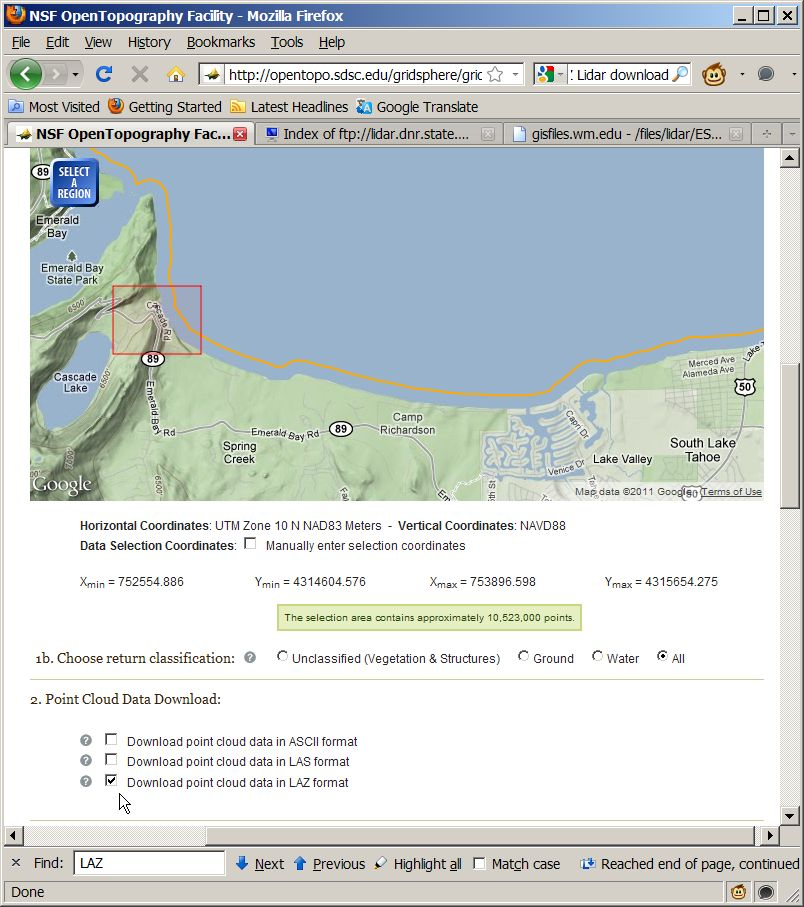
\includegraphics[width=0.65\textwidth]{images/open_topo}}}
    \uncover<2->{\put(100,-50){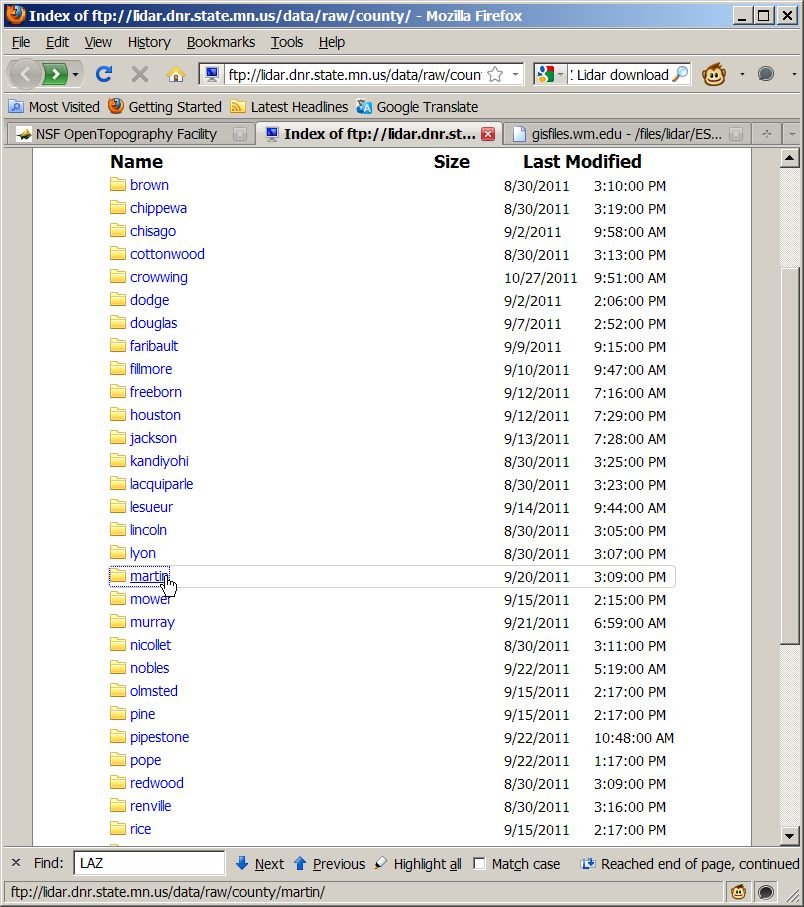
\includegraphics[width=0.65\textwidth]{images/minnesota}}}
    \uncover<3->{\put(100,-50){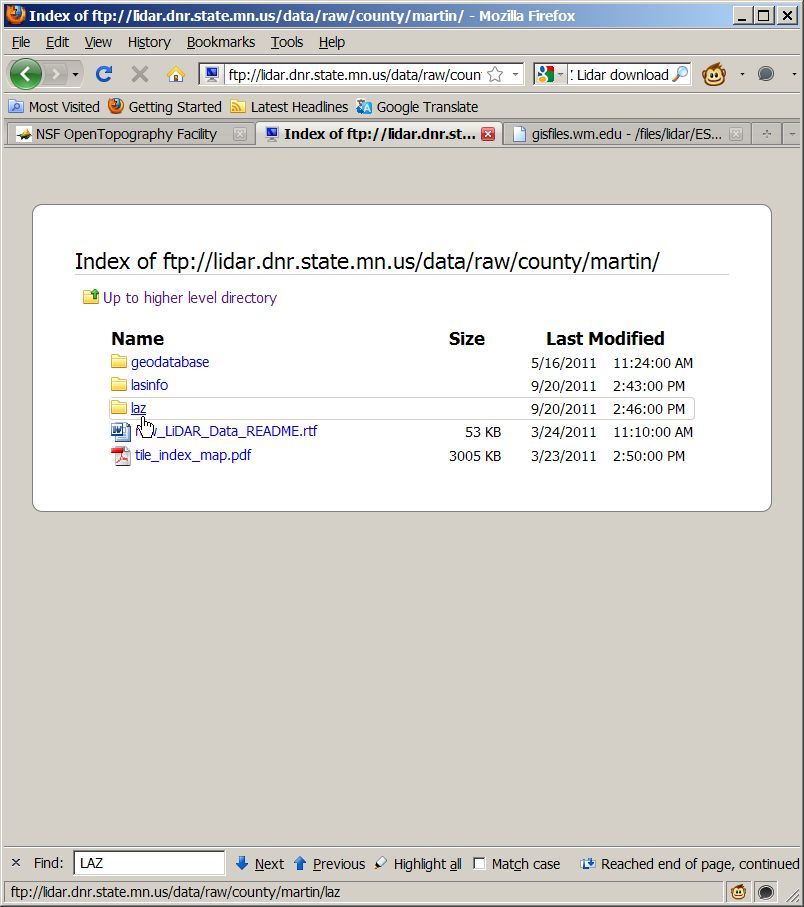
\includegraphics[width=0.65\textwidth]{images/minnesota_martin}}}
    \uncover<4->{\put(100,-50){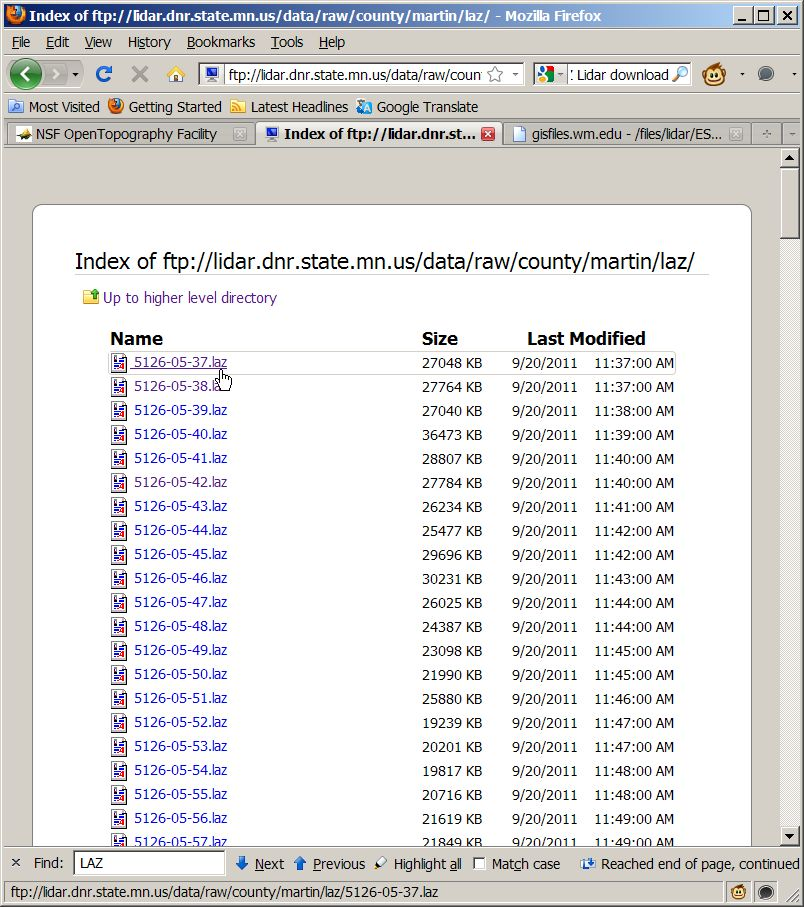
\includegraphics[width=0.65\textwidth]{images/minnesota_laz}}}
    \uncover<5->{\put(100,-50){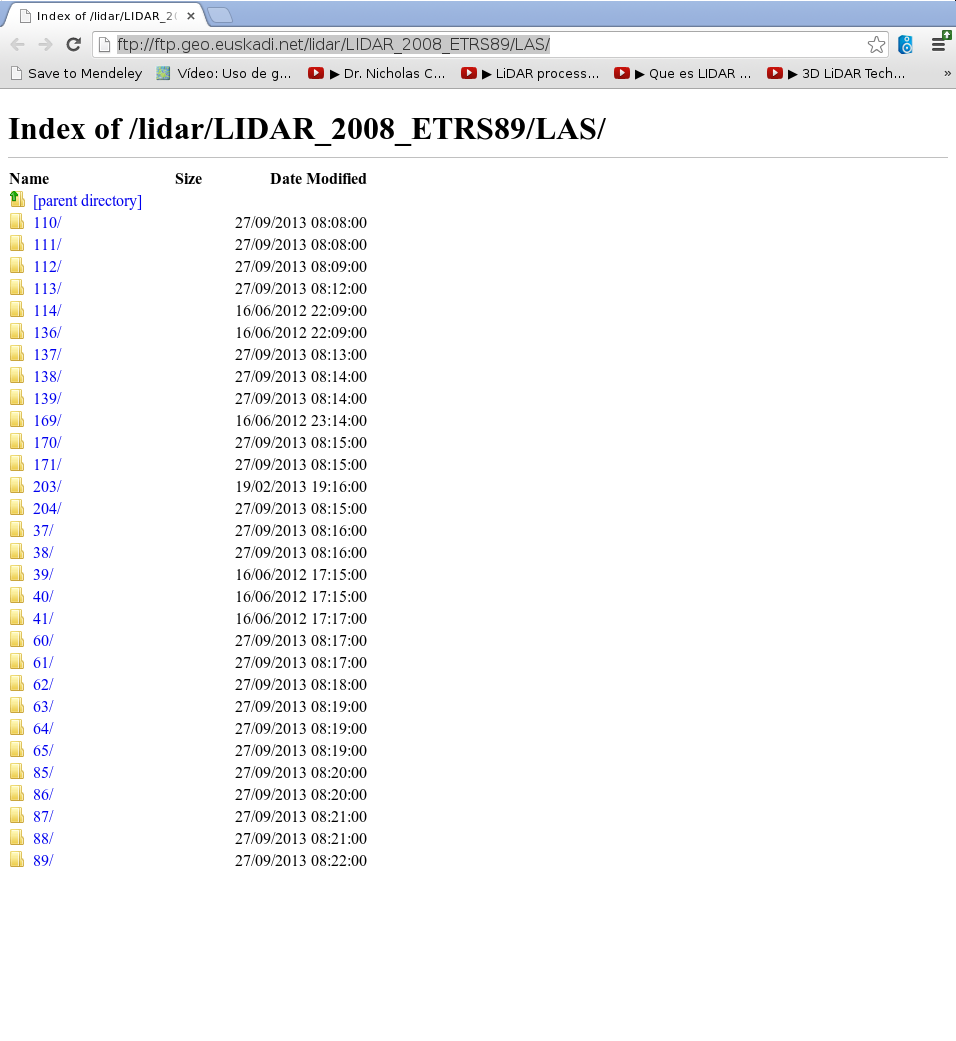
\includegraphics[width=0.65\textwidth]{images/paisvasco_data}}}
  \end{picture}
\end{frame}
%%==================================================================S
\section[DTM]{Modelos Digitales del Terreno}
%%==================================================================F
\begin{frame}
  \frametitle{Modelos Digitales del Terreno (DTM)}
  \begin{beamerboxesrounded}[shadow=true]{Definición}
    Teóricamente sería una representación continua, $f$, del terreno en un
    cierto área local. Dadas las coordenadas planimétricas de un punto,
    $\mathbf{p}=(x,y)$, y su valor altimétrico asociado, $z$, la representación
    \alert{2.5D} del terreno, sería: $z=f(x,y)$
  \end{beamerboxesrounded}
  \begin{itemize}
    \item \alert{2.5D $\ne$ 3D}
      \begin{itemize}
        \item $z_1 = \mathbf{p}(x,y)$; $z_2 = \mathbf{p}(x,y)$ \alert{¡!}
        \item Puentes y pasos elevados $\Rightarrow$ \alert{No se consideran}
      \end{itemize}
  \end{itemize}
\end{frame}
%%==================================================================F
\begin{frame}
  \frametitle{Tipos de Modelos digitales}
  \begin{minipage}{.4\textwidth}
  \begin{enumerate}
    \item Realidad
    \item Modelo Digital de Superficie (DSM)
    \item Modelo de Edificios (DBM)
    \item Modelo Digital del Terreno (DTM)
  \end{enumerate}
  \end{minipage}
  \begin{minipage}{.55\textwidth}
    \includegraphics[height=0.20\textheight]{images/realidad}\\
    \includegraphics[height=0.20\textheight]{images/dsm}\\
    \includegraphics[height=0.20\textheight]{images/dbm}\\
    \includegraphics[height=0.20\textheight]{images/dtm}
  \end{minipage}
\end{frame}
%%==================================================================F
\begin{frame}
  \frametitle{DTM Vs. DSM}
  \begin{enumerate}
    \item \alert{DTM}
    \begin{itemize}
      \item Se busca un suavizado de la superficie
      \item Se utilizan los últimos ecos para filtrar
    \end{itemize}
    \item \alert{DSM}
    \begin{itemize}
      \item Se busca resaltar los detalles
      \item Se utilizan los primeros impulsos
      \item Errores en observaciones groseras $\Rightarrow$ \alert{Limpiar}
      \item Objetos temporales (coches, gruas\ldots) $\Rightarrow$ \alert{Limpiar}
    \end{itemize}
  \end{enumerate}
\end{frame}
%%==================================================================F
\begin{frame}
  \frametitle{nDSM}
    \begin{itemize}
      \item \alert{nDSM = DSM - DSM}
    \end{itemize}
    \begin{center}
      \includegraphics[width=0.30\textwidth]{images/n_dsm}~--~
      \includegraphics[width=0.30\textwidth]{images/n_dtm}~$\Rightarrow$~
      \includegraphics[width=0.30\textwidth]{images/n_ndsm}~
    \end{center}
\end{frame}
%%==================================================================Sb
\subsection[Ráster]{Estructuras regulares}
%%==================================================================F
\begin{frame}
  \frametitle{Continuo Vs. Discreto}
  \begin{enumerate}
    \item Interesa almacenar la representación del DTM una vez conocida
    \item Opción: definición de la funcion $z = f(x,y)$ + el área
      \begin{itemize}
        \item[\tickYes] Realmente continuo
        \item[\tickNo] No siempre es conocida
        \item[\tickNo] No es algo estándar
      \end{itemize}
    \item Discretización en un intervalos regulares
      \begin{itemize}
        \item[\tickNo] No es continuo
        \item[\tickYes] Fácilmente almacenable
        \item[\tickYes] Existen multitud de formatos ``estándar''
      \end{itemize}
  \end{enumerate}
\end{frame}
%%==================================================================F
\begin{frame}
  \frametitle{Raster Vs. Mallado}
  \begin{enumerate}
    \item \alert{Ráster} 
      \begin{itemize}
        \item Cada celda representa la altura de todo el área que cubre la celda
      \end{itemize}
    \item \alert{Malla}
      \begin{itemize}
        \item Representa la información de altura en puntos regularmente ordenados
        \item Cada altura es la evaluación de $f$ en cada punto $(x,y)$ de la
          malla
        \item Interpolación, aproximación (inverso de la distancia pesada),
          mínimos cuadrados móviles, kriging, etc,\ldots
      \end{itemize}
    \item Son uno el dual del otro
    \item Se suelen confundir
  \end{enumerate}
\end{frame}
%%==================================================================F
\begin{frame}
  \frametitle{Ráster}
  \begin{center}
        \includegraphics[height=0.60\textheight]{images/raster}
  \end{center}
\end{frame}
%%==================================================================F
\begin{frame}
  \frametitle{Malla}
  \begin{center}
        \includegraphics[height=0.60\textheight]{images/mallado}
  \end{center}
\end{frame}
%%==================================================================F
\begin{frame}
  \frametitle{Malla híbrida}
  \begin{center}
        \includegraphics[height=0.60\textheight]{images/malla_breaklines}
  \end{center}
\end{frame}
%%==================================================================Sb
\subsection{TIN}
%%==================================================================F
\begin{frame}
  \frametitle{TIN}
  \begin{enumerate}
    \item \alert{TIN}: \emph{Triangulated irregular network}
    \item Los puntos topológicamente vecinos deben guardar unas reglas
      geométricas: \alert{Triangulación de Delaunay}
    \item Permiten también modelos híbridos con líneas de ruptura
    \item Formatos estándares
  \end{enumerate}
\end{frame}
%%==================================================================F
\begin{frame}
  \frametitle{Triangulación}
  \begin{center}
        \includegraphics[height=0.60\textheight]{images/triangulacion}
  \end{center}
\end{frame}
%%==================================================================F
\begin{frame}
  \frametitle{TIN}
  \begin{center}
        \includegraphics[height=0.60\textheight]{images/tin_dem}
  \end{center}
\end{frame}
%%==================================================================F
\begin{frame}
  \frametitle{Triangulación de Delaunay}
  \begin{beamerboxesrounded}[shadow=true]{Definición: \emph{Triangulación de
    Delaunay}}
    Sea $P$ un conjunto de puntos en el \alert{plano}, se dice que $T$ es una
    \alert{\emph{Triangulación de Delaunay}} $\Leftrightarrow$ cualquier círculo que
    circunscriba cualquier triángulo de $T$ no encierra ningún otro punto de $P$
    \end{beamerboxesrounded}
  \begin{enumerate}
    \item La mejor aproximación posible genera triángulos regulares
    \item En cualquier caso: maximiza el menor ángulo de cada triángulo
  \begin{center}
        \includegraphics[height=0.15\textwidth]{images/triang_regular}
  \end{center}
  \end{enumerate}
\end{frame}
%%==================================================================F
\begin{frame}
  \frametitle{Triangulación de Delaunay}
  \begin{beamerboxesrounded}[shadow=true]{Propiedad 1}
    Sea $P$ un conjunto de puntos en el plano, entonces tres puntos $p_i, p_j$ y
    $p_k$ son vértices del mismo triángulo de la triangulación de Delaunay de $P
    \Leftrightarrow$ la circunferencia que pasa por los tres puntos no encierra
    ningún punto de $P$
  \end{beamerboxesrounded}
  \begin{center}
  \includegraphics[height=0.20\textwidth]{images/propiedad1}
  \end{center}
\end{frame}
%%==================================================================F
\begin{frame}
  \frametitle{Triangulación de Delaunay}
  \begin{beamerboxesrounded}[shadow=true]{Propiedad 2}
    Sea $P$ un conjunto de puntos en el plano, entonces, dos puntos, $p_i$ y
    $p_j$ forman un segmento de la triangulación de Delaunay de $P
    \Leftrightarrow$ existe una circunferencia que contiene a ambos pero no
    encierra ningún punto de $P$
  \end{beamerboxesrounded}
  \begin{center}
  \includegraphics[height=0.20\textwidth]{images/propiedad2}
  \end{center}
\end{frame}
%%==================================================================F
\begin{frame}
  \frametitle{Diagrama de Voronoi}
  \begin{center}
  \includegraphics[height=0.20\textwidth]{images/voronoi}
  \end{center}
\end{frame}
%%==================================================================Sb
\subsection[Calidad]{Calidad de los DTM}
%%==================================================================F
\begin{frame}
  \frametitle{Calidad de los DTM}
  \begin{enumerate}
    \item \alert{Calidad de los datos}
      \begin{itemize}
        \item Describe la calidad de los datos de entrada
      \end{itemize}
    \item \alert{Calidad del modelo}
      \begin{itemize}
        \item Describe la calidad del modelo final generado
      \end{itemize}
  \end{enumerate}
\end{frame}
%%==================================================================F
\begin{frame}
  \frametitle{Calidad de los datos}
  \begin{enumerate}
    \item Capa de densidad de puntos
      \begin{itemize}
        \item Permite identificar zonas con escasez de datos
        \item Ofrece información sobre las posibles interpolaciones y
          extrapolaciones
      \end{itemize}
    \item Capa de distancia entre puntos
      \begin{itemize}
        \item Parecida al mapa de densidad
        \item Permite conocer zona con pocos puntos
        \item Da información sobre la distancia del vecino más próximo
      \end{itemize}
    \item Fuentes de datos
      \begin{itemize}
        \item Da información sobre la presencia de distintos tipos de inputs:
          ALS, TLS, fotogrametría, etc\ldots
      \end{itemize}
    \item Mapa de precisión de las fuentes de datos
      \begin{itemize}
        \item Da información sobre la mejor o peor precisión de los datos
      \end{itemize}
  \end{enumerate}
\end{frame}
%%==================================================================F
\begin{frame}
  \frametitle{Pasadas}
    \begin{center}
      \only<1>{\includegraphics[width=0.55\textwidth]{images/pasadas}}
      \only<2>{\includegraphics[width=0.55\textwidth]{images/pasadas_shademap}}
    \end{center}
\end{frame}
%%==================================================================F
\begin{frame}
  \frametitle{Mapa de densidades}
    \begin{center}
      \includegraphics[width=0.45\textwidth]{images/densidad}
    \end{center}
\end{frame}
%%==================================================================F
\begin{frame}
  \frametitle{Densidad de pasadas}
    \begin{center}
      \includegraphics[width=0.45\textwidth]{images/densidad_pasadas}
    \end{center}
\end{frame}
%%==================================================================F
\begin{frame}
  \frametitle{Calidad de los datos}
  \begin{enumerate}
    \item Información sobre la consistencia de los datos
    \item ¿La calidad del filtro? (terreno vs. no-terreno)
      \begin{itemize}
        \item Introducen errores en zonas complejas
        \item No hay un modo preciso de calcular la calidad de la clasificación
        \item Suelen estar basado en la \emph{\alert{experiencia práctica}}
      \end{itemize}
    \item Vegetación baja
      \begin{itemize}
        \item Dificil decir si un eco pertenece al terreno
        \item Introducen un \alert{sesgo sistemático} en altura
        \item Se necesitan información adicional
      \end{itemize}
  \end{enumerate}
\end{frame}
%%==================================================================F
\begin{frame}
  \frametitle{Calidad del modelo}
  \begin{enumerate}
    \item Calidad \alert{interior}
      \begin{itemize}
        \item Es la calidad del modelo respecto a las \alert{propios datos}
      \end{itemize}
    \item Calidad \alert{exterior}
      \begin{itemize}
        \item Es la calidad del modelo respecto a \alert{puntos de control
          externos (GCP)}
      \end{itemize}
  \end{enumerate}
\end{frame}
%%==================================================================F
\begin{frame}
  \frametitle{Calidad interior}
  \begin{enumerate}
    \item Es la calidad del modelo respecto a las propios datos
    \item Se aplica la ley propagación de los errores
    \item \alert{RMSE} (raíz del error cuadrático medio)
      \[ \mathrm{RMSE(\widehat\theta)}=\sqrt{\mathrm{E}\left[(\widehat\theta - \theta)^2\right]}\]
    \item Representa la precisión del proceso de generación del DTM 
    \item Ayuda a identificar áreas con diferencias significativas entre
      modelo y datos
  \end{enumerate}
\end{frame}
%%==================================================================F
\begin{frame}
  \frametitle{Calidad exterior}
  \begin{enumerate}
    \item Es la calidad del modelo respecto a puntos de control externos (GCP)
      \begin{itemize}
        \item Los GCP no tienen que usarse durante la generación del DTM
        \item Tienen que ser mucho más precisos que los datos de input
      \end{itemize}
    \item Describe tanto los inputs como el proceso del modelado
    \item Generalmente se utiliza \alert{RMSE}
    \item Estimación en \alert{altura} [Karel y Kraus (2006)]
        \[\sigma_z[\mathrm{cm}] = \pm\left(\dfrac{6}{\sqrt{n}} +
        30\tan(\alpha)\right)\]
      \begin{itemize}
        \item $n$: densidad puntual (pts/m$^2$)
        \item $\tan(\alpha)$: inclinación del terreno
      \end{itemize}
  \end{enumerate}
\end{frame}
%%==================================================================Sc
\subsection{Reducción de los datos}
%%==================================================================F
\begin{frame}
  \frametitle{Densidad puntual}
  \begin{enumerate}
    \item \alert{Todavía} es importante una reducción de la densidad
      puntual\alert{!}
    \item Escaneo: $100$ KHz $\Rightarrow$ \alert{$\approx$ 10
      pts/$\mathrm{m}^2$} $\Rightarrow$ Alta resolución en el DTM
    \item Problemas de almacenamiento y procesado
    \item Necesaria una reducción de la densidad
    \item Métodos
      \begin{itemize}
        \item Cambio de la estructura del DTM
        \item Sin cambio de la estructura del DTM
      \end{itemize}
  \end{enumerate}
\end{frame}
%%==================================================================F
\begin{frame}
  \frametitle{Remuestreo}
  \begin{enumerate}
    \item Métodos estándar en el procesado de imágenes digitales
    \item Menor resolución con celdas más grandes
    \item El valor del píxel nuevo se deriva de las celdas originales
    \item \alert{Ventajas}
      \begin{itemize}
        \item Aplicable también para mallas
        \item Muy rápido y mantiene la estructura
      \end{itemize}
    \item \alert{Desventajas}
      \begin{itemize}
        \item No son adaptativos: presentan problemas con diferencia de alturas
         \begin{itemize}
           \item Raster adaptativos locales: \alert{poco usados}
         \end{itemize}
      \end{itemize}
  \end{enumerate}
\end{frame}
%%==================================================================F
\begin{frame}
  \frametitle{TIN's}
  \begin{enumerate}
    \item \alert{Purga de puntos}
      \begin{itemize}
        \item Considera el TIN completo 
        \item elimina puntos paso a paso
      \end{itemize}
    \item \alert{Aproximación por subdivisión}
      \begin{itemize}
        \item Empieza con un TIN aproximado
        \item Utiliza algoritmos \alert{divide y vencerás} hasta alcanzar cierto
          criterio
      \end{itemize}
    \item Necesitan teselar el TIN 
    \item Poco eficaces \alert{justo después} del filtrado
      \begin{itemize}
        \item Errores en las observaciones y en zonas de solape (poco eficaces)
        \item Interpolación suavizada de alta resolución de los puntos
      \end{itemize}
  \end{enumerate}
\end{frame}
%%==================================================================Sc
\section[Procesado]{Procesado de los datos}
%%==================================================================F
\begin{frame}
  \frametitle{Flujo de Trabajo}
    \tikzstyle{decision} = [diamond, draw, fill=blue!20, 
        text width=4.5em, text badly centered, node distance=1.25cm, inner sep=0pt]
    \tikzstyle{block} = [rectangle, draw, fill=blue!20,
        % text width=7em, 
        text centered, rounded corners, minimum height=2em]
    \tikzstyle{line} = [draw, -latex']
    \tikzstyle{cloud} = [draw, ellipse,fill=red!20, node distance=2cm,
        minimum height=2em]
  \begin{center}
    \begin{tikzpicture}[node distance=.75cm, auto]
        \tiny
        % Place nodes
        \node [block] (init)
        {\begin{tabular}{c}
          {Datos LiDAR}
        \end{tabular}
        };
        \node [decision, below of=init] (ntiles) {Teselar?};
        \node [block, below of=ntiles, node distance=1.15cm] (merge)
        {\begin{tabular}{c}
          Unir archivos
         \end{tabular}
        };
        \node [block, right of=ntiles, node distance=2.5cm] (tiling)
        {\begin{tabular}{c}
          Crear teselas
         \end{tabular}
        };
        \node [block, below of=merge] (rmnoise)
        {\begin{tabular}{c}
          Eliminar ruido
         \end{tabular}
        };
        \node [decision, below of=rmnoise] (classify) {Clasificar?};
        \node [block, right of=classify, node distance=2.5cm] (filter)
        {\begin{tabular}{c}
          Clasificar terreno
         \end{tabular}
        };
        \node [block, right of=filter, node distance=2.5cm] (height)
        {\begin{tabular}{c}
          Calcular alturas
         \end{tabular}
        };
        \node [block, below of=filter, node distance=1.15cm] (interpolate)
        {\begin{tabular}{c}
          Interpolar
         \end{tabular}
        };
        % \node [block, below of=height, node distance=1.15cm] (interpolate2)
        % {\begin{tabular}{c}
        %   Interpolar
        %  \end{tabular}
        % };
        \node [decision, below of=interpolate] (metrics) {Métricas?};
        \node [block, left of=metrics, node distance=2.5cm] (metric)
        {\begin{tabular}{c}
          Calcular Métricas
         \end{tabular}
        };
        \node [block, below of=metrics, node distance=1.15cm] (stop) 
        {\begin{tabular}{c}
          {Final}
        \end{tabular}
        };

        \node [cloud, right of=metrics] (dsm) {\textbf{DSM}};
        \node [cloud, right of=dsm, node distance=2.5cm] (dtm) {\textbf{DTM} and \textbf{CHM}};

        % Draw edges
        \path [line] (init) -- (ntiles);
        \path [line] (ntiles) -- node [near start] {uno} (merge);
        \path [line] (ntiles) -- node [near start] {muchos} (tiling);
        \path [line] (tiling) |- (rmnoise);
        \path [line] (merge) -- (rmnoise);
        \path [line] (rmnoise) -- (classify);
        \path [line] (classify) -- node [near start] {si} (filter);
        \path [line] (classify) |- node [near start] {no} (interpolate);
        \path [line] (filter) -- (height);
        \path [line] (height) |- (interpolate);
        \path [line] (interpolate) -- (metrics);
        \path [line] (metrics) -- node [near start] {si} (metric);
        \path [line] (metrics) -- node [near start] {no} (stop);
        \path [line] (metric) |- (stop);
        \path [line] (interpolate) -- (dsm);
        \path [line] (interpolate) -| (dtm);
        % \path [line] (height) -| (dtm);
    \end{tikzpicture}
  \end{center}
\end{frame}
%%==================================================================Sc
\section[Filtros]{Filtros ALS}
%%==================================================================F
\begin{frame}
  \frametitle{Filtros}
  \begin{enumerate}
    \item Es necesario extraer información de la nube de puntos: terreno,
      no-terreno.
    \item Paso imprescindible para la generación de DTM
    \item Clasificación en diferentes categorías:
      \begin{itemize}
        \item Terreno
        \item Edificio
        \item Vegetación
        \item Pasos elevados, etc\ldots
      \end{itemize}
    \item Las idea subyacente son también aplicables otras técnicas como TLS,
      pero con características diferentes (densidad).
  \end{enumerate}
\end{frame}
%%==================================================================FIN
\begin{frame}
 \titlepage
\end{frame}

%================================================================== Logo On/Off
\LogoOff

%==================================================================FRONT PAGE AND TOC
% For article only
\mode<presentation:0>{\thispagestyle{empty}\maketitle}

% For presentation only
\mode<presentation| article:0| handout:0>{
    \begin{frame}<article:0>[label=portada]
    \titlepage
    \end{frame}%Fin del frame
}

% For handout only
\mode<handout>{
  \begin{frame}[label=portada]
    \maketitle
  \end{frame}
}

%% TABLE OF CONTENTS
\begin{frame}[label=toc]
    \mode<article:0>{\frametitle{Contents}}
    \mode<presentation>{\small}
    \tableofcontents%[hidesubsections]
\end{frame}

%%==================================================================S INTRODUCTION
\section[ALS]{\textquestiondown Qué es el LiDAR aéreo?}
%%==================================================================Sb
\subsection{Principios}
%%==================================================================F 
\begin{frame}
 \frametitle{Principios del LiDAR aéreo}
 \begin{enumerate}
   \item El LiDAR aéreo (Airborne Laser Scanner, \alert{ALS}) es la combinación de:
    	\begin{itemize}
    	 \item \alert{Escaner Laser}
    	 \item \alert{GPS}, que nos da la posición del sensor.
    	 \item \alert{IMU}, que nos da nuestra orientación del avión.
    	\end{itemize}
   \item La posición con respecto al sensor de un punto en tierra se determina por:
     \begin{itemize}
       \item El \alert{tiempo} que tarda cada impulso desde que es emitido hasta que es recibido.
       \item El \alert{ángulo} medido desde el nadir en el cual ha sido emitido el rayo.
     \end{itemize}
   \item La posición relativa combinada con la posición global (\alert{GPS}) y la orientación (\alert{IMU}) nos permiten calcular las coordenadas (X,Y,Z) en el punto medido en tierra en un sistema de posicionamiento global (WGS84)
 \end{enumerate}
\end{frame}
%%==================================================================Sb
\subsection{Características}
%%==================================================================F
\begin{frame}[label=lidar_charact]
   \frametitle{Características del ALS}
   \begin{enumerate}
     	\item \alert{Alta precisión} tanto en la componente planimétrica como en la altrimétrica
     	\item \alert{Alta resolución} debido a la frecuencia de medición.
     	\item \alert{Monoscópica} y casi \alert{nadiral} $\Rightarrow$ permite observar el terreno incluso en zonas de gran vegetación
   \end{enumerate}
\end{frame}
%%==================================================================Sb
\subsection{Primer y último impulso}
%%==================================================================F 
\begin{frame}
  \frametitle{LiDAR}
    \begin{center}
      \only<1>{\includegraphics[width=0.95\textheight]{images/rebote}}
      \only<2>{\includegraphics[width=0.95\textheight]{images/rebotes}}
    \end{center}
\end{frame}
%%==================================================================F
\begin{frame}[label=firstlast1]
    \frametitle{Primer y último impulso}
    \begin{enumerate}
      \item Debido a la divergencia del láser, pueden recibirse \alert{más de un eco} para el mismo rayo.
    	\item Los sensores actuales son capaces de medir al menos dos retornos: \alert{primero} y \alert{último}
    	\item Normalmente se producen por: \alert{bordes} de edificios o \alert{vegetación}
    \end{enumerate}
    \begin{center}
      \includegraphics[height=0.35\textheight]{images/roof}~
      \includegraphics[height=0.35\textheight]{images/tree}
    \end{center}
\end{frame}
%%==================================================================F 
\begin{frame}
    \frametitle{\textquestiondown Para qué sirve?}
    \begin{enumerate}
     \item Una diferencia considerable entre el primer y último impulso puede ser una pista para detectar vegetación y otros objetos: edificios, puentes, tendidos eléctricos...
     \item Los últimos impulsos tienen más probabilidad de ser terreno
     	\begin{itemize}
     	   \item Primer impulso: creación de Modelo Digital de Superficie (\alert{DSM})
     	   \item \'Ultimo impulso: determinación de Modelo Digital del Terreno (\alert{DTM})
     	\end{itemize}
     \item Hay pocas posibilidades de, sin hacer ningún análisis, distinguir entre un punto \alert{objeto} y uno \alert{terreno}.
    \end{enumerate}
\end{frame}
%%==================================================================S
\section[Datos]{Datos LiDAR}
%%==================================================================F
\begin{frame}
  \frametitle{Estándares}
    \begin{center}
      \includegraphics[width=0.75\textwidth]{images/standards}
    \end{center}
  \tiny
  \begin{itemize}
    \item \alert{SITUACIÓN}: Hay 14 estándares diferentes
    \item 14?! Ridículo! Necesitamos desarrollar un estándar universal que cubra todos los posibles casos de uso
    \item \alert{SITUACIÓN}: Hay 15 estándares diferentes
  \end{itemize}
\end{frame}
%%==================================================================F 
\pgfdeclareimage[width=0.7\textwidth]{las}{images/las_format}
\begin{frame}
\frametitle{Estándar binario \emph{LAS} del ASPRS:}
\begin{itemize}
 \item Encabezado público
 \item Registros de longitud variable
 \item Puntos: X, Y, Z, Intensidad, clasificación, dirección de la pasada del vuelo,...
    \begin{center}
  \begin{tikzpicture}
        \pgftext[bottom,left,at={\pgfpointxy{0}{0}}]{\pgfuseimage{las}}
  \end{tikzpicture}
   \end{center}
 \item Para un conversor \alert{abierto} del estándar \emph{LAS}:
\beamergotobutton{\url{http://liblas.org/}}
\end{itemize}
\end{frame}
%%==================================================================F 
\defverbatim[colored]\laszip{
  \begin{lstlisting}[style=shell]
    $ laszip lidar.las lidar.laz
    $ laszip lidar.laz lidar_copy.las
  \end{lstlisting}
}
\begin{frame}
\frametitle{Estándar binario \emph{LAZ}}
\begin{enumerate}
  \item Compresión de archivos .LAS sin \alert{pérdida}
  \item 7\% - 20\% del tamaño del archivo original
  \item Formato LAS comprimido \beamergotobutton{\url{http://www.laszip.org/}}
  \item Ejemplo:
    \laszip
\end{enumerate}
\end{frame}
%%==================================================================F 
\frame[containsverbatim]{%
  \frametitle {Estándar binario SPD}
  \begin{itemize}
    \item Encabezado público
    \item Ficheros indexados
    \item Puntos: X, Y, Z, Intensidad, clasificación, dirección de la pasada del vuelo,...
    \item Procesa datos \alert{\emph{full waveform}}
    \item Página: \beamergotobutton{\url{http://www.spdlib.org/}}
  \end{itemize}
}
%%==================================================================F 
\frame[containsverbatim]{%
  \frametitle {Posible formato ASCII}
  \begin{center}
  \begin{verbatim}
              X         Y        Z
          513628.82 5403190.04 291.40
          513628.85 5403191.47 291.24
          513628.95 5403192.93 294.31
          513628.99 5403194.45 294.17
          513628.97 5403196.05 291.26
          513629.01 5403197.58 291.24
          513629.05 5403199.10 291.25
          513629.09 5403200.53 291.26
                        ...
  \end{verbatim}
  \end{center}
}
%%==================================================================F 
\begin{frame}
  \frametitle{¡Datos LIBRES!}
  \begin{itemize}
    \item \beamergotobutton{\url{http://www.lidar-online.com/products-list.php}}
    \item \beamergotobutton{\url{http://opentopo.sdsc.edu/gridsphere/gridsphere?cid=databases}}
    \item \beamergotobutton{\url{http://opentopography.org/}}
    \item \beamergotobutton{\url{http://liblas.org/samples/}}
    \item \beamergotobutton{\url{http://www.csc.noaa.gov/digitalcoast/data/chartstopobathy/download}}
    \item \beamergotobutton{\url{ftp://ftp.lmic.state.mn.us/pub/data/elevation/lidar/}}
    \item \beamergotobutton{\url{https://www.lidar-online.com/}}
  \end{itemize}
      Muchos más en:
  \begin{itemize}
    \item \beamergotobutton{\url{http://laszip.org/}}
  \end{itemize}
\end{frame}
%%==================================================================F 
\begin{frame}
  \frametitle{Descarga de archivos .LAZ}
  \begin{minipage}{0.35\textwidth}
  \begin{enumerate}[<+->]
    \item Open Topography
    \item Minnesota DNR
    \item<5> País Vasco
  \end{enumerate}
  \end{minipage}
  \begin{picture}(300,100)
    \uncover<1->{\put(100,-50){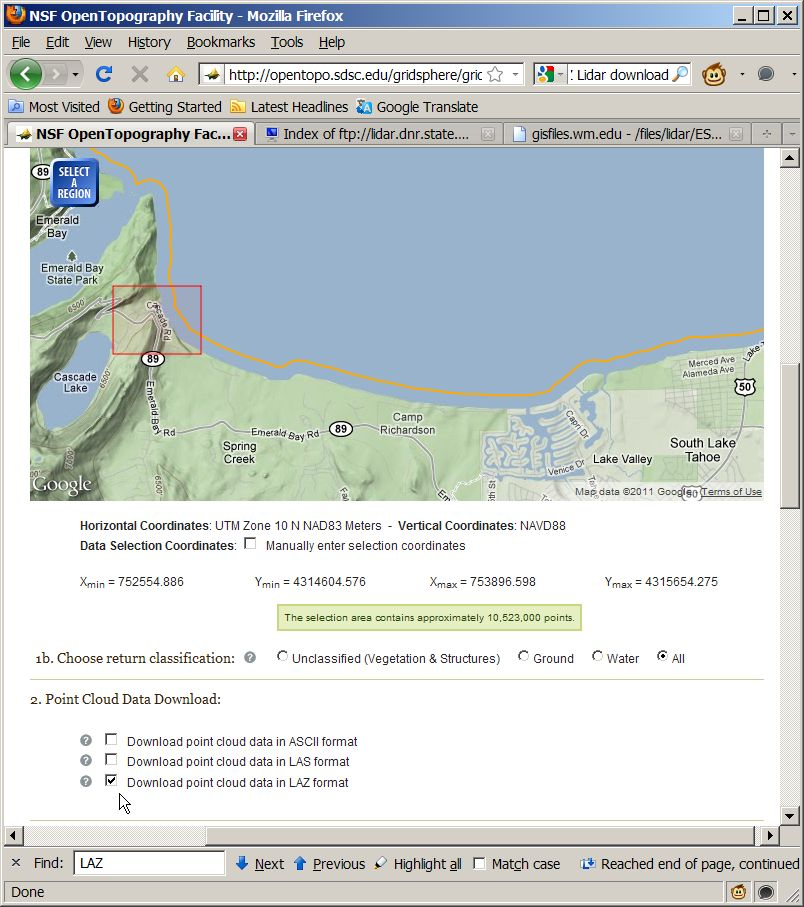
\includegraphics[width=0.65\textwidth]{images/open_topo}}}
    \uncover<2->{\put(100,-50){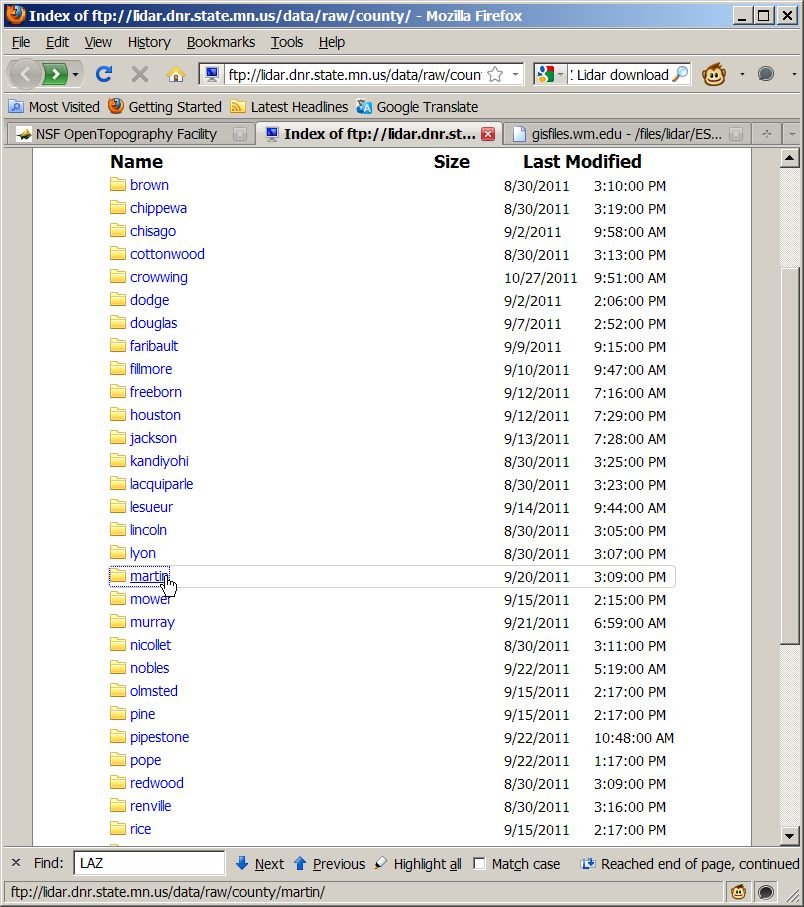
\includegraphics[width=0.65\textwidth]{images/minnesota}}}
    \uncover<3->{\put(100,-50){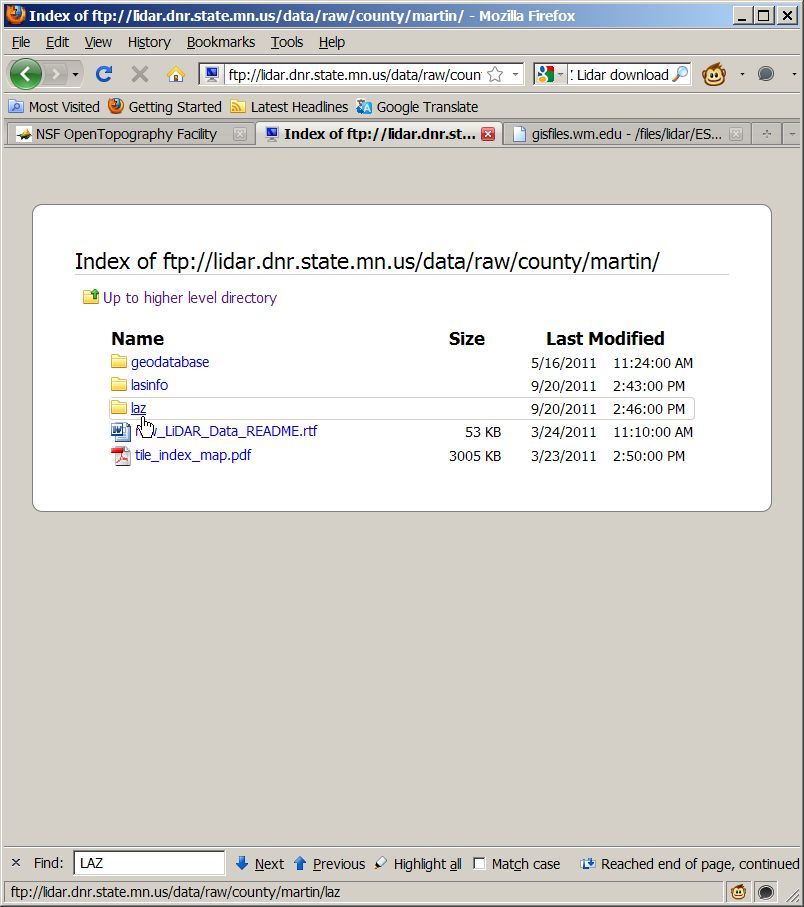
\includegraphics[width=0.65\textwidth]{images/minnesota_martin}}}
    \uncover<4->{\put(100,-50){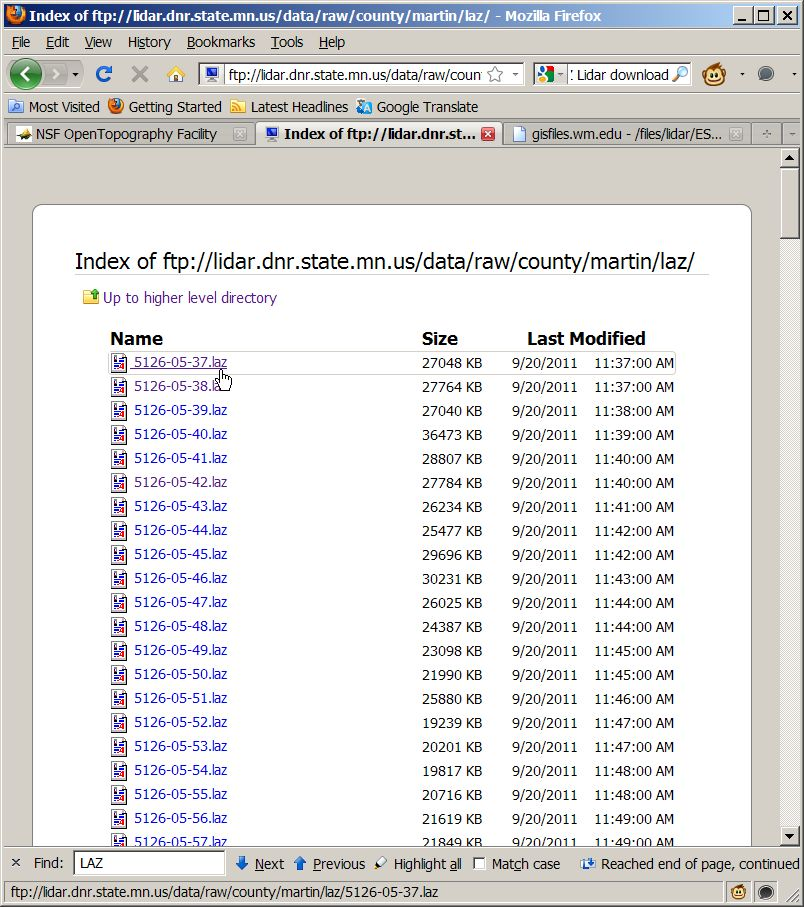
\includegraphics[width=0.65\textwidth]{images/minnesota_laz}}}
    \uncover<5->{\put(100,-50){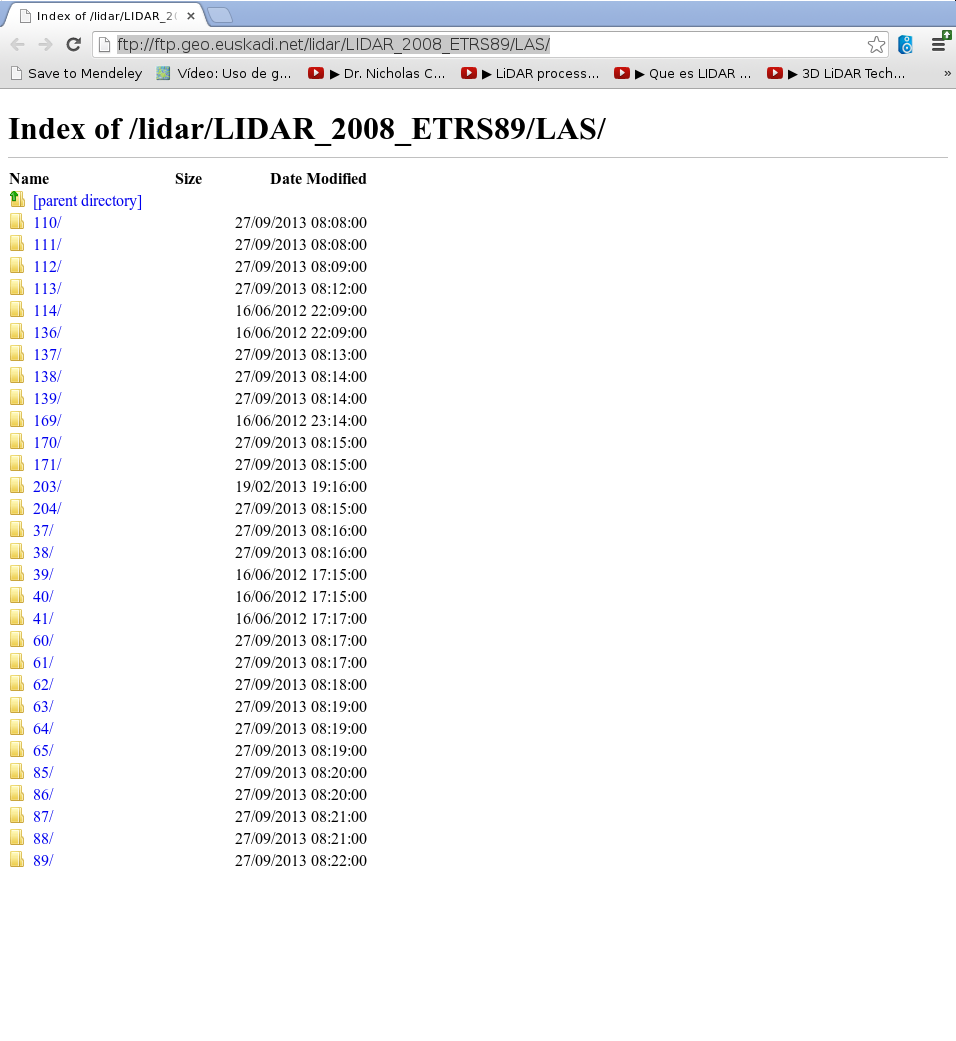
\includegraphics[width=0.65\textwidth]{images/paisvasco_data}}}
  \end{picture}
\end{frame}
%%==================================================================S
\section[DTM]{Modelos Digitales del Terreno}
%%==================================================================F
\begin{frame}
  \frametitle{Modelos Digitales del Terreno (DTM)}
  \begin{beamerboxesrounded}[shadow=true]{Definición}
    Teóricamente sería una representación continua, $f$, del terreno en un
    cierto área local. Dadas las coordenadas planimétricas de un punto,
    $\mathbf{p}=(x,y)$, y su valor altimétrico asociado, $z$, la representación
    \alert{2.5D} del terreno, sería: $z=f(x,y)$
  \end{beamerboxesrounded}
  \begin{itemize}
    \item \alert{2.5D $\ne$ 3D}
      \begin{itemize}
        \item $z_1 = \mathbf{p}(x,y)$; $z_2 = \mathbf{p}(x,y)$ \alert{¡!}
        \item Puentes y pasos elevados $\Rightarrow$ \alert{No se consideran}
      \end{itemize}
  \end{itemize}
\end{frame}
%%==================================================================F
\begin{frame}
  \frametitle{Tipos de Modelos digitales}
  \begin{minipage}{.4\textwidth}
  \begin{enumerate}
    \item Realidad
    \item Modelo Digital de Superficie (DSM)
    \item Modelo de Edificios (DBM)
    \item Modelo Digital del Terreno (DTM)
  \end{enumerate}
  \end{minipage}
  \begin{minipage}{.55\textwidth}
    \includegraphics[height=0.20\textheight]{images/realidad}\\
    \includegraphics[height=0.20\textheight]{images/dsm}\\
    \includegraphics[height=0.20\textheight]{images/dbm}\\
    \includegraphics[height=0.20\textheight]{images/dtm}
  \end{minipage}
\end{frame}
%%==================================================================F
\begin{frame}
  \frametitle{DTM Vs. DSM}
  \begin{enumerate}
    \item \alert{DTM}
    \begin{itemize}
      \item Se busca un suavizado de la superficie
      \item Se utilizan los últimos ecos para filtrar
    \end{itemize}
    \item \alert{DSM}
    \begin{itemize}
      \item Se busca resaltar los detalles
      \item Se utilizan los primeros impulsos
      \item Errores en observaciones groseras $\Rightarrow$ \alert{Limpiar}
      \item Objetos temporales (coches, gruas\ldots) $\Rightarrow$ \alert{Limpiar}
    \end{itemize}
  \end{enumerate}
\end{frame}
%%==================================================================F
\begin{frame}
  \frametitle{nDSM}
    \begin{itemize}
      \item \alert{nDSM = DSM - DSM}
    \end{itemize}
    \begin{center}
      \includegraphics[width=0.30\textwidth]{images/n_dsm}~--~
      \includegraphics[width=0.30\textwidth]{images/n_dtm}~$\Rightarrow$~
      \includegraphics[width=0.30\textwidth]{images/n_ndsm}~
    \end{center}
\end{frame}
%%==================================================================Sb
\subsection[Ráster]{Estructuras regulares}
%%==================================================================F
\begin{frame}
  \frametitle{Continuo Vs. Discreto}
  \begin{enumerate}
    \item Interesa almacenar la representación del DTM una vez conocida
    \item Opción: definición de la funcion $z = f(x,y)$ + el área
      \begin{itemize}
        \item[\tickYes] Realmente continuo
        \item[\tickNo] No siempre es conocida
        \item[\tickNo] No es algo estándar
      \end{itemize}
    \item Discretización en un intervalos regulares
      \begin{itemize}
        \item[\tickNo] No es continuo
        \item[\tickYes] Fácilmente almacenable
        \item[\tickYes] Existen multitud de formatos ``estándar''
      \end{itemize}
  \end{enumerate}
\end{frame}
%%==================================================================F
\begin{frame}
  \frametitle{Raster Vs. Mallado}
  \begin{enumerate}
    \item \alert{Ráster} 
      \begin{itemize}
        \item Cada celda representa la altura de todo el área que cubre la celda
      \end{itemize}
    \item \alert{Malla}
      \begin{itemize}
        \item Representa la información de altura en puntos regularmente ordenados
        \item Cada altura es la evaluación de $f$ en cada punto $(x,y)$ de la
          malla
        \item Interpolación, aproximación (inverso de la distancia pesada),
          mínimos cuadrados móviles, kriging, etc,\ldots
      \end{itemize}
    \item Son uno el dual del otro
    \item Se suelen confundir
  \end{enumerate}
\end{frame}
%%==================================================================F
\begin{frame}
  \frametitle{Ráster}
  \begin{center}
        \includegraphics[height=0.60\textheight]{images/raster}
  \end{center}
\end{frame}
%%==================================================================F
\begin{frame}
  \frametitle{Malla}
  \begin{center}
        \includegraphics[height=0.60\textheight]{images/mallado}
  \end{center}
\end{frame}
%%==================================================================F
\begin{frame}
  \frametitle{Malla híbrida}
  \begin{center}
        \includegraphics[height=0.60\textheight]{images/malla_breaklines}
  \end{center}
\end{frame}
%%==================================================================Sb
\subsection{TIN}
%%==================================================================F
\begin{frame}
  \frametitle{TIN}
  \begin{enumerate}
    \item \alert{TIN}: \emph{Triangulated irregular network}
    \item Los puntos topológicamente vecinos deben guardar unas reglas
      geométricas: \alert{Triangulación de Delaunay}
    \item Permiten también modelos híbridos con líneas de ruptura
    \item Formatos estándares
  \end{enumerate}
\end{frame}
%%==================================================================F
\begin{frame}
  \frametitle{Triangulación}
  \begin{center}
        \includegraphics[height=0.60\textheight]{images/triangulacion}
  \end{center}
\end{frame}
%%==================================================================F
\begin{frame}
  \frametitle{TIN}
  \begin{center}
        \includegraphics[height=0.60\textheight]{images/tin_dem}
  \end{center}
\end{frame}
%%==================================================================F
\begin{frame}
  \frametitle{Triangulación de Delaunay}
  \begin{beamerboxesrounded}[shadow=true]{Definición: \emph{Triangulación de
    Delaunay}}
    Sea $P$ un conjunto de puntos en el \alert{plano}, se dice que $T$ es una
    \alert{\emph{Triangulación de Delaunay}} $\Leftrightarrow$ cualquier círculo que
    circunscriba cualquier triángulo de $T$ no encierra ningún otro punto de $P$
    \end{beamerboxesrounded}
  \begin{enumerate}
    \item La mejor aproximación posible genera triángulos regulares
    \item En cualquier caso: maximiza el menor ángulo de cada triángulo
  \begin{center}
        \includegraphics[height=0.15\textwidth]{images/triang_regular}
  \end{center}
  \end{enumerate}
\end{frame}
%%==================================================================F
\begin{frame}
  \frametitle{Triangulación de Delaunay}
  \begin{beamerboxesrounded}[shadow=true]{Propiedad 1}
    Sea $P$ un conjunto de puntos en el plano, entonces tres puntos $p_i, p_j$ y
    $p_k$ son vértices del mismo triángulo de la triangulación de Delaunay de $P
    \Leftrightarrow$ la circunferencia que pasa por los tres puntos no encierra
    ningún punto de $P$
  \end{beamerboxesrounded}
  \begin{center}
  \includegraphics[height=0.20\textwidth]{images/propiedad1}
  \end{center}
\end{frame}
%%==================================================================F
\begin{frame}
  \frametitle{Triangulación de Delaunay}
  \begin{beamerboxesrounded}[shadow=true]{Propiedad 2}
    Sea $P$ un conjunto de puntos en el plano, entonces, dos puntos, $p_i$ y
    $p_j$ forman un segmento de la triangulación de Delaunay de $P
    \Leftrightarrow$ existe una circunferencia que contiene a ambos pero no
    encierra ningún punto de $P$
  \end{beamerboxesrounded}
  \begin{center}
  \includegraphics[height=0.20\textwidth]{images/propiedad2}
  \end{center}
\end{frame}
%%==================================================================F
\begin{frame}
  \frametitle{Diagrama de Voronoi}
  \begin{center}
  \includegraphics[height=0.20\textwidth]{images/voronoi}
  \end{center}
\end{frame}
%%==================================================================Sb
\subsection[Calidad]{Calidad de los DTM}
%%==================================================================F
\begin{frame}
  \frametitle{Calidad de los DTM}
  \begin{enumerate}
    \item \alert{Calidad de los datos}
      \begin{itemize}
        \item Describe la calidad de los datos de entrada
      \end{itemize}
    \item \alert{Calidad del modelo}
      \begin{itemize}
        \item Describe la calidad del modelo final generado
      \end{itemize}
  \end{enumerate}
\end{frame}
%%==================================================================F
\begin{frame}
  \frametitle{Calidad de los datos}
  \begin{enumerate}
    \item Capa de densidad de puntos
      \begin{itemize}
        \item Permite identificar zonas con escasez de datos
        \item Ofrece información sobre las posibles interpolaciones y
          extrapolaciones
      \end{itemize}
    \item Capa de distancia entre puntos
      \begin{itemize}
        \item Parecida al mapa de densidad
        \item Permite conocer zona con pocos puntos
        \item Da información sobre la distancia del vecino más próximo
      \end{itemize}
    \item Fuentes de datos
      \begin{itemize}
        \item Da información sobre la presencia de distintos tipos de inputs:
          ALS, TLS, fotogrametría, etc\ldots
      \end{itemize}
    \item Mapa de precisión de las fuentes de datos
      \begin{itemize}
        \item Da información sobre la mejor o peor precisión de los datos
      \end{itemize}
  \end{enumerate}
\end{frame}
%%==================================================================F
\begin{frame}
  \frametitle{Pasadas}
    \begin{center}
      \only<1>{\includegraphics[width=0.55\textwidth]{images/pasadas}}
      \only<2>{\includegraphics[width=0.55\textwidth]{images/pasadas_shademap}}
    \end{center}
\end{frame}
%%==================================================================F
\begin{frame}
  \frametitle{Mapa de densidades}
    \begin{center}
      \includegraphics[width=0.45\textwidth]{images/densidad}
    \end{center}
\end{frame}
%%==================================================================F
\begin{frame}
  \frametitle{Densidad de pasadas}
    \begin{center}
      \includegraphics[width=0.45\textwidth]{images/densidad_pasadas}
    \end{center}
\end{frame}
%%==================================================================F
\begin{frame}
  \frametitle{Calidad de los datos}
  \begin{enumerate}
    \item Información sobre la consistencia de los datos
    \item ¿La calidad del filtro? (terreno vs. no-terreno)
      \begin{itemize}
        \item Introducen errores en zonas complejas
        \item No hay un modo preciso de calcular la calidad de la clasificación
        \item Suelen estar basado en la \emph{\alert{experiencia práctica}}
      \end{itemize}
    \item Vegetación baja
      \begin{itemize}
        \item Dificil decir si un eco pertenece al terreno
        \item Introducen un \alert{sesgo sistemático} en altura
        \item Se necesitan información adicional
      \end{itemize}
  \end{enumerate}
\end{frame}
%%==================================================================F
\begin{frame}
  \frametitle{Calidad del modelo}
  \begin{enumerate}
    \item Calidad \alert{interior}
      \begin{itemize}
        \item Es la calidad del modelo respecto a las \alert{propios datos}
      \end{itemize}
    \item Calidad \alert{exterior}
      \begin{itemize}
        \item Es la calidad del modelo respecto a \alert{puntos de control
          externos (GCP)}
      \end{itemize}
  \end{enumerate}
\end{frame}
%%==================================================================F
\begin{frame}
  \frametitle{Calidad interior}
  \begin{enumerate}
    \item Es la calidad del modelo respecto a las propios datos
    \item Se aplica la ley propagación de los errores
    \item \alert{RMSE} (raíz del error cuadrático medio)
      \[ \mathrm{RMSE(\widehat\theta)}=\sqrt{\mathrm{E}\left[(\widehat\theta - \theta)^2\right]}\]
    \item Representa la precisión del proceso de generación del DTM 
    \item Ayuda a identificar áreas con diferencias significativas entre
      modelo y datos
  \end{enumerate}
\end{frame}
%%==================================================================F
\begin{frame}
  \frametitle{Calidad exterior}
  \begin{enumerate}
    \item Es la calidad del modelo respecto a puntos de control externos (GCP)
      \begin{itemize}
        \item Los GCP no tienen que usarse durante la generación del DTM
        \item Tienen que ser mucho más precisos que los datos de input
      \end{itemize}
    \item Describe tanto los inputs como el proceso del modelado
    \item Generalmente se utiliza \alert{RMSE}
    \item Estimación en \alert{altura} [Karel y Kraus (2006)]
        \[\sigma_z[\mathrm{cm}] = \pm\left(\dfrac{6}{\sqrt{n}} +
        30\tan(\alpha)\right)\]
      \begin{itemize}
        \item $n$: densidad puntual (pts/m$^2$)
        \item $\tan(\alpha)$: inclinación del terreno
      \end{itemize}
  \end{enumerate}
\end{frame}
%%==================================================================Sc
\subsection{Reducción de los datos}
%%==================================================================F
\begin{frame}
  \frametitle{Densidad puntual}
  \begin{enumerate}
    \item \alert{Todavía} es importante una reducción de la densidad
      puntual\alert{!}
    \item Escaneo: $100$ KHz $\Rightarrow$ \alert{$\approx$ 10
      pts/$\mathrm{m}^2$} $\Rightarrow$ Alta resolución en el DTM
    \item Problemas de almacenamiento y procesado
    \item Necesaria una reducción de la densidad
    \item Métodos
      \begin{itemize}
        \item Cambio de la estructura del DTM
        \item Sin cambio de la estructura del DTM
      \end{itemize}
  \end{enumerate}
\end{frame}
%%==================================================================F
\begin{frame}
  \frametitle{Remuestreo}
  \begin{enumerate}
    \item Métodos estándar en el procesado de imágenes digitales
    \item Menor resolución con celdas más grandes
    \item El valor del píxel nuevo se deriva de las celdas originales
    \item \alert{Ventajas}
      \begin{itemize}
        \item Aplicable también para mallas
        \item Muy rápido y mantiene la estructura
      \end{itemize}
    \item \alert{Desventajas}
      \begin{itemize}
        \item No son adaptativos: presentan problemas con diferencia de alturas
         \begin{itemize}
           \item Raster adaptativos locales: \alert{poco usados}
         \end{itemize}
      \end{itemize}
  \end{enumerate}
\end{frame}
%%==================================================================F
\begin{frame}
  \frametitle{TIN's}
  \begin{enumerate}
    \item \alert{Purga de puntos}
      \begin{itemize}
        \item Considera el TIN completo 
        \item elimina puntos paso a paso
      \end{itemize}
    \item \alert{Aproximación por subdivisión}
      \begin{itemize}
        \item Empieza con un TIN aproximado
        \item Utiliza algoritmos \alert{divide y vencerás} hasta alcanzar cierto
          criterio
      \end{itemize}
    \item Necesitan teselar el TIN 
    \item Poco eficaces \alert{justo después} del filtrado
      \begin{itemize}
        \item Errores en las observaciones y en zonas de solape (poco eficaces)
        \item Interpolación suavizada de alta resolución de los puntos
      \end{itemize}
  \end{enumerate}
\end{frame}
%%==================================================================Sc
\section[Procesado]{Procesado de los datos}
%%==================================================================F
\begin{frame}
  \frametitle{Flujo de Trabajo}
    \tikzstyle{decision} = [diamond, draw, fill=blue!20, 
        text width=4.5em, text badly centered, node distance=1.25cm, inner sep=0pt]
    \tikzstyle{block} = [rectangle, draw, fill=blue!20,
        % text width=7em, 
        text centered, rounded corners, minimum height=2em]
    \tikzstyle{line} = [draw, -latex']
    \tikzstyle{cloud} = [draw, ellipse,fill=red!20, node distance=2cm,
        minimum height=2em]
  \begin{center}
    \begin{tikzpicture}[node distance=.75cm, auto]
        \tiny
        % Place nodes
        \node [block] (init)
        {\begin{tabular}{c}
          {Datos LiDAR}
        \end{tabular}
        };
        \node [decision, below of=init] (ntiles) {Teselar?};
        \node [block, below of=ntiles, node distance=1.15cm] (merge)
        {\begin{tabular}{c}
          Unir archivos
         \end{tabular}
        };
        \node [block, right of=ntiles, node distance=2.5cm] (tiling)
        {\begin{tabular}{c}
          Crear teselas
         \end{tabular}
        };
        \node [block, below of=merge] (rmnoise)
        {\begin{tabular}{c}
          Eliminar ruido
         \end{tabular}
        };
        \node [decision, below of=rmnoise] (classify) {Clasificar?};
        \node [block, right of=classify, node distance=2.5cm] (filter)
        {\begin{tabular}{c}
          Clasificar terreno
         \end{tabular}
        };
        \node [block, right of=filter, node distance=2.5cm] (height)
        {\begin{tabular}{c}
          Calcular alturas
         \end{tabular}
        };
        \node [block, below of=filter, node distance=1.15cm] (interpolate)
        {\begin{tabular}{c}
          Interpolar
         \end{tabular}
        };
        % \node [block, below of=height, node distance=1.15cm] (interpolate2)
        % {\begin{tabular}{c}
        %   Interpolar
        %  \end{tabular}
        % };
        \node [decision, below of=interpolate] (metrics) {Métricas?};
        \node [block, left of=metrics, node distance=2.5cm] (metric)
        {\begin{tabular}{c}
          Calcular Métricas
         \end{tabular}
        };
        \node [block, below of=metrics, node distance=1.15cm] (stop) 
        {\begin{tabular}{c}
          {Final}
        \end{tabular}
        };

        \node [cloud, right of=metrics] (dsm) {\textbf{DSM}};
        \node [cloud, right of=dsm, node distance=2.5cm] (dtm) {\textbf{DTM} and \textbf{CHM}};

        % Draw edges
        \path [line] (init) -- (ntiles);
        \path [line] (ntiles) -- node [near start] {uno} (merge);
        \path [line] (ntiles) -- node [near start] {muchos} (tiling);
        \path [line] (tiling) |- (rmnoise);
        \path [line] (merge) -- (rmnoise);
        \path [line] (rmnoise) -- (classify);
        \path [line] (classify) -- node [near start] {si} (filter);
        \path [line] (classify) |- node [near start] {no} (interpolate);
        \path [line] (filter) -- (height);
        \path [line] (height) |- (interpolate);
        \path [line] (interpolate) -- (metrics);
        \path [line] (metrics) -- node [near start] {si} (metric);
        \path [line] (metrics) -- node [near start] {no} (stop);
        \path [line] (metric) |- (stop);
        \path [line] (interpolate) -- (dsm);
        \path [line] (interpolate) -| (dtm);
        % \path [line] (height) -| (dtm);
    \end{tikzpicture}
  \end{center}
\end{frame}
%%==================================================================Sc
\section[Filtros]{Filtros ALS}
%%==================================================================F
\begin{frame}
  \frametitle{Filtros}
  \begin{enumerate}
    \item Es necesario extraer información de la nube de puntos: terreno,
      no-terreno.
    \item Paso imprescindible para la generación de DTM
    \item Clasificación en diferentes categorías:
      \begin{itemize}
        \item Terreno
        \item Edificio
        \item Vegetación
        \item Pasos elevados, etc\ldots
      \end{itemize}
    \item Las idea subyacente son también aplicables otras técnicas como TLS,
      pero con características diferentes (densidad).
  \end{enumerate}
\end{frame}
%%==================================================================FIN
\begin{frame}
 \titlepage
\end{frame}

\end{document}
